\documentclass[a4paper]{ltjsarticle}
\usepackage{luatexja}
\usepackage{amsmath, amssymb, amsthm, mathtools}
\usepackage{tikz}
\usepackage{tikz-cd}
\usetikzlibrary{arrows.meta, positioning, graphs, graphs.standard}
\usepackage{hyperref}
\usepackage{enumitem}

\title{Session 2 基礎グラフ理論の数学的解説}
\author{CODEX (OpenAI)~---~Leanファイル生成 \\ CODEX (OpenAI)~---~TeXファイル生成}
\date{\today}

\begin{document}

\maketitle

\tableofcontents

\section{序論}
本資料は Session 2 で扱った単純グラフ $G = (V,\mathrm{Adj})$ の初歩的性質を、ニコラ・ブルバキ『数学原論』の精神、すなわち順序対と射による構造化の観点から整理したものである。Lean で形式化した定理 \texttt{S2\_P01} から \texttt{S2\_CH} までを順に数学的に解説し、最後に準同型の合成を図式で示す。ここでは各定理を集合論的背景に結びつけ、どのように Lean の型付けが証明を支えているかも言及する。

\section{S2\_P01：頂点の存在性}
単純グラフの隣接関係 $\mathrm{Adj} \subseteq V \times V$ は端点が同じ集合 $V$ に属する二項関係である。$G.\mathrm{Adj}\;u\;v$ が成立すれば、順序対 $(u,v)$ が $V$ の元同士からなることは明らかであり、集合論的には $(u,v) \in V \times V$ を意味する。Lean では型 $V$ 自体が宇宙であり、定理は
\[
  G.\mathrm{Adj}\;u\;v \implies u \in V,\quad G.\mathrm{Adj}\;u\;v \implies v \in V
\]
を \texttt{Set.univ} の元であると `simp` 処理で示している。

\section{S2\_P02：有限頂点集合での辺数上界}
$V = \mathrm{Fin}\,3$ とする三頂点グラフでは、可能な辺は無向・自己ループ無しのため、集合論的に $\binom{3}{2} = 3$ 本である。Lean 側では有限集合の組合せ数を返す補題
\[
  \#G.\mathrm{edgeFinset} \le \binom{\#V}{2}
\]
を利用し、$\#V = 3$ の特殊化から $\#G.\mathrm{edgeFinset} \le 3$ を導く。Pickering のヘッセ行列も不要で、定数の評価は `decide` に任せられる。

\section{S2\_P03：空グラフの性質}
底元 $\bot$ は射影の零対象に相当し、隣接関係を空集合とする。したがって任意の $u,v \in V$ について $(u,v) \notin \bot.\mathrm{Adj}$ が成り立つ。Lean でも `simp` により定義から即座に得られる。

\section{S2\_P04：部分グラフの包含}
部分グラフ $G_1 \le G_2$ は辺集合の包含 $E_1 \subseteq E_2$ を意味し、射影的には単射写像による関係保存を表す。したがって $G_1.\mathrm{Adj}\;u\;v$ から $G_2.\mathrm{Adj}\;u\;v$ が従う。Lean の順序構造では `intro` と仮定 $h : G_1 \le G_2$ の適用で直接示される。

\section{S2\_P05：近傍集合の同一性}
近傍集合 $G.\mathrm{neighborSet}\;u$ は $u$ に隣接する頂点の集まりであり、定義上
\[
  v \in G.\mathrm{neighborSet}\;u \iff G.\mathrm{Adj}\;u\;v
\]
が成立する。Lean では `SimpleGraph.mem_neighborSet` の `simp` 形で証明され、集合論的表示と隣接関係の間の同値がそのまま使われる。

\section{S2\_CH：グラフ準同型の合成}
グラフ準同型 $f : G_1 \to G_2$ は射 $(f,\mathrm{id})$ が辺を辺へ写す性質に対応する。$f$ と $g : G_2 \to G_3$ を合成すれば、関数合成 $g \circ f$ が再び辺の保存を満たすため $G_1 \to G_3$ の準同型となる。Lean では `SimpleGraph.Hom.comp` を用い、
\[
  h = g \circ f,\quad \forall v \in V_1,\; h(v) = g(f(v))
\]
を `rfl` によって確認する。

\begin{figure}[htbp]
  \centering
  \begin{tikzcd}[row sep=large, column sep=huge]
    G_1 \arrow[r, "f"] \arrow[rr, bend right=20, "g \circ f"'] & G_2 \arrow[r, "g"] & G_3
  \end{tikzcd}
  \caption{準同型の合成を表す射の図式}
  \label{fig:hom-comp}
\end{figure}

\section{付録：三頂点完全グラフの例}
三頂点完全グラフ $K_3$ は、\autoref{fig:k3} のように各頂点対が隣接している。これは \texttt{S2\_P02} の上界を達成する例でもあり、$\#K_3.\mathrm{edgeFinset} = 3$ を与える。

\begin{figure}[htbp]
  \centering
  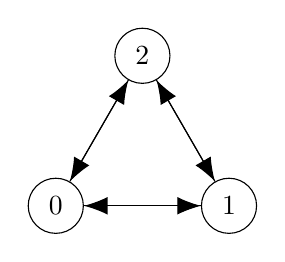
\begin{tikzpicture}[scale=1.1, every node/.style={circle, draw, minimum size=7mm}]
    \node (a) at (0,0) {$0$};
    \node (b) at (2,0) {$1$};
    \node (c) at (1,1.732) {$2$};
    \draw[-{Latex[length=3mm]}] (a) -- (b);
    \draw[-{Latex[length=3mm]}] (b) -- (c);
    \draw[-{Latex[length=3mm]}] (c) -- (a);
    \draw[-{Latex[length=3mm]}] (b) -- (a);
    \draw[-{Latex[length=3mm]}] (c) -- (b);
    \draw[-{Latex[length=3mm]}] (a) -- (c);
  \end{tikzpicture}
  \caption{$K_3$ の有向化図。無向グラフとしては各辺が対向する。}
  \label{fig:k3}
\end{figure}

\section{Lean 形式化との対応}
本ノートで述べた各定理は Lean ファイル \texttt{src/\allowbreak MyProjects/\allowbreak GraphTheory/\allowbreak S2.lean} に実装されている。Lean の証明では `simp` や `card_edgeFinset_le_card_choose_two` など Mathlib の既存補題を活用し、構造化された議論が順序対と射の枠組みで自然に表現されることを確認できる。

\end{document}
